\section{Parallel Gaussian Channels}
If there are  $k$ common power constaint, guassian channels (NWAGN : non-white additive Guassian Noise channel) which are considered to be independent and in parallel where different frequency is represented by each parallel channel. Distributing power among all channels to maximise the channel capacity would be the ultimate goal.
\\
\begin{center}
	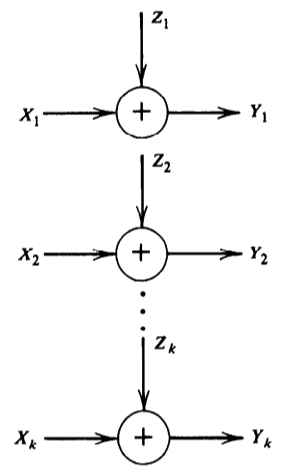
\includegraphics[scale=0.5]{Diagrams/parallel_guassian_channels.png}
\end{center} 
Recalling basics from Guassian channels, sum of Input and Guassian noise constitutes the output of each channel.Similarly, from the above figure for channel $j$ , it would be:
%
\begin{eqnarray}
    Y_j = X_j + Z_j, \quad j = 1, 2, \dots, k,
\end{eqnarray}
%

%
with
\begin{eqnarray}
    Z_j \sim \mathcal{N}(0, N_j),
\end{eqnarray}
%
and as mentioned above , there is a constaint on power \textit{i.e.} common power and the channels including the noise is independent.The constaint can be described as:
%
\begin{eqnarray}
    \mathbb{E} \sum_{j=1}^{k} X_j^2 \leq P
\end{eqnarray}
%
information capacity of Channel C is given by:
%
\begin{eqnarray}
    C = \max_{f(x_1, x_2, \dots, x_k) : \sum \mathbb{E} X_j^2 \leq P} I(X_1, X_2, \dots, X_k ; Y_1, Y_2, \dots, Y_k)
\end{eqnarray}
%
To achieve the goal of {max Capacity} , need to observe the distribution which makes it possible . It is well known that C is supreme of all achievable rates ,and since all channels are independent ,
\\
\( Z_1, Z_2, \dots, Z_k \) are independent,
%
\begin{eqnarray}
    I(X_1, X_2, \dots, X_k; Y_1, Y_2, \dots, Y_k) &=& h(Y_1, Y_2, \dots, Y_k) - h(Y_1, Y_2, \dots, Y_k | X_1, X_2, \dots, X_k) \\
    &=& h(Y_1, Y_2, \dots, Y_k) - h(Z_1, Z_2, \dots, Z_k) \\
    &=& \sum h(Y_j) - \sum h(Z_j) \\
    &\leq& \sum \frac{1}{2} \log \left( 1 + \frac{P_j}{N_j} \right),
\end{eqnarray}
%
where \( P_j = \mathbb{E} X_j^2 \), and \( \sum P_j = P \). 
LHS = RHS  is possible when,
%
\begin{eqnarray}
    (X_1, X_2, \dots, X_k) \sim \mathcal{N} \left( 0, \begin{pmatrix} P_1 & 0 & \dots & 0 \\ 0 & P_2 & \dots & 0 \\ \vdots & \vdots & \ddots & \vdots \\ 0 & 0 & \dots & P_k \end{pmatrix} \right).
\end{eqnarray}
%
In order to maximise Capacity , power allotment in the constaint \( \sum P_j = P \) needs to be found.By Lagrange multipliers,
%
\begin{eqnarray}
    J(P_1, \dots, P_k) = \sum \frac{1}{2} \log \left( 1 + \frac{P_j}{N_j} \right) + \lambda \left( \sum P_j \right)
\end{eqnarray}
%
by differentiating above {wrt} \( P_j \), 
%
\begin{eqnarray}
    \frac{1}{2} \frac{1}{P_j + N_j} + \lambda = 0,
\end{eqnarray}
%
in other terms,
%
\begin{eqnarray}
    P_j = \nu - N_j.
\end{eqnarray}
%
Due to the fact that \( P_j \)'s must be positive,Kuhn-Tucker conditions can be used to find $v$ such that capacity is maximum.
%
\begin{eqnarray}
    P_j = (\nu - N_j)^+
\end{eqnarray}
%
above $(x)^+$ shows non-negative of $x$,

\[
(x)^+ = 
\begin{cases}
x, & \text{if } x \geq 0, \\
0, & \text{if } x < 0.
\end{cases}
\]
%
The picture below gives an graphical representation of a solution , power is alloted to channels as signal power increases from 0 , power is put into channels which are noiser . Like this Power is distributed into various bins and is referred to as $"Water-Filling"$ process.
\begin{center}
	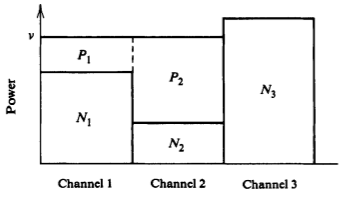
\includegraphics[scale=0.5]{Diagrams/parallel_guassian_channels_solution.png}
\end{center} 
